\documentclass{beamer}
%\documentclass[handout]{beamer}

\usepackage[latin1]{inputenc}
%\usepackage[french]{babel}

\beamertemplatenavigationsymbolsempty

\definecolor{kwblue}{rgb}{0.67,0.12,0.92}
\definecolor{ceruleanblue}{rgb}{0, 0.48, 0.65}
\definecolor{lightpink}{rgb}{1., 0.71, 0.75}
\definecolor{lightblue}{rgb}{0.8,0.8,1}
\definecolor{lightred}{rgb}{1,0.8,0.8}

\let\emph\alert
\newcommand{\coeurs}{c\oe urs}

\begin{document}

\title{Functory : Une biblioth�que de calcul distribu� \\ pour
  Objective Caml}
\author[Jean-Christophe]{Jean-Christophe Filli\^atre \& Kalyan Krishnamani}
\date{JFLA, 31 janvier 2011}

\begin{frame}
  \titlepage
  \pgfimage[height=8mm]{cnrs-logo2}\hfill
  \pgfimage[height=6mm]{saclay}\hfill
  \pgfimage[height=10mm]{lrilogo}\hfill
  \pgfimage[height=8mm]{upsudlogo}
\end{frame}

\begin{frame}\frametitle{Motivation}
  \begin{itemize}
  \item Why platform: a set of tools for deductive program verification
  \item generates numerous verification conditions (VCs)
  \item discharged by various automated theorem provers
  \item typically takes hours to complete
  \end{itemize}


  \begin{itemize}
  \item a few multi-core machines at our disposal
  \item how to make the best possible use of them?
  \end{itemize}
\end{frame}

\begin{frame}\frametitle{A Distributed Computing Library}

  requirements
  \begin{itemize}
  \item ideally in Ocaml
  \item fault tolerance
  \item user-friendly API
  \end{itemize}
\end{frame}

\begin{frame}\frametitle{Basic Design}
  inspired by Google's Map/Reduce (OSDI 2004)


  \begin{center}
    \includegraphics{master_workers_1.mps}
  \end{center}
\end{frame}

\begin{frame}\frametitle{Interface}

  \begin{ocaml}
  val compute : 
    worker:('a -> 'b) -> 
    master:('a * 'c -> 'b -> ('a * 'c) list) -> 
    ('a * 'c) list -> 
    unit
  \end{ocaml}



  \begin{itemize}
  \item a task has type \ocaml{'a * 'c}, its result has type \ocaml{'b}
  \item a completed task may generate new tasks
  \item the whole computation returns when there is no more task
  \end{itemize}
\end{frame}

% TODO: insert a small example here?

\begin{frame}\frametitle{Simple Implementations}
  \begin{description}
  \item[sequential]
    \begin{itemize}
    \item used for debugging and comparison
    \end{itemize}


  \item[multi-core] 
    \begin{itemize}
    \item to utilize multiple cores on a single machine
    \end{itemize}
  \end{description}
\end{frame}

\begin{frame}\frametitle{Network Implementation}
  based on
  \begin{itemize}
  \item TCP/IP client/server architecture
  \item Ocaml's marshaling capabilities
  \end{itemize}
  
  \vfill
  marshaling considerations
  \begin{enumerate}
  \item \emph{same binary}: we can marshal closures
  \item \emph{same version of Ocaml}: we can only marshal values
  \item \emph{otherwise}: we only marshal strings
  \end{enumerate}
\end{frame}

\begin{frame}\frametitle{Three Network Implementations}
\emph{same binary}
\begin{ocaml}
val compute : (* same as before *) ...
\end{ocaml}



\emph{same version of Caml}
    \begin{ocaml}
val Worker.compute : ('a -> 'b) -> unit
val Master.compute : 
  ('a * 'c -> 'b -> ('a * 'c) list) ->
  ('a * 'c) list -> unit
\end{ocaml}



\emph{otherwise}
    \begin{ocaml}
val Worker.compute : (string -> string) -> unit
val Master.compute : 
  (string * 'c -> string -> (string * 'c) list) ->
  (string * 'c) list -> unit
\end{ocaml}
\end{frame}

\begin{frame}\frametitle{Implementation Details: Cores}

  simply uses \texttt{Unix.fork} (no control over scheduling)

  \begin{ocaml}
  open Cores
  let () = set_number_of_cores 4
  \end{ocaml}

  \begin{center}
    \includegraphics{master_workers_cores.mps}
  \end{center}

  master maintains a queue of pending tasks
\end{frame}

\begin{frame}\frametitle{Implementation Details: Netwok}

  \begin{ocaml}
  open Network
  let () = declare_workers ~n:3 "moloch"
  let () = declare_workers ~n:2 "orcus"
  \end{ocaml}

  \begin{center}
    \includegraphics{master_workers_network.mps}
  \end{center}
  each worker behaves as a server, the master being the client
\end{frame}

\begin{frame}\frametitle{Protocol}
  \only<1,5>{master sends a task to a worker}
  \only<2>{worker computes and sends back a result}
  \only<3-4>{master and workers exchange \emph{ping}/\emph{pong} messages}
  \only<6>{in case of a disconnection...}
  \only<7>{the task is \emph{rescheduled} to another worker}
  \only<8>{whenever one completes...}
  \only<9>{the other one is stopped}
  \only<10>{the master is notified when a computation fails}
  \only<11>{at the very end, the master may ask the workers to stop}
  \vfill
  \begin{center}
    \only<1,5>{\includegraphics{master_workers_assign.mps}}
    \only<2>{\includegraphics{master_workers_completed.mps}}
    \only<3>{\includegraphics{master_workers_ping.mps}}
    \only<4>{\includegraphics{master_workers_pong.mps}}
    \only<6>{\includegraphics{master_workers_disconnection.mps}}
    \only<7>{\includegraphics{master_workers_assign_2.mps}}
    \only<8>{\includegraphics{master_workers_completed_2.mps}}
    \only<9>{\includegraphics{master_workers_kill.mps}}
    \only<10>{\includegraphics{master_workers_aborted.mps}}
    \only<11>{\includegraphics{master_workers_stop.mps}}
  \end{center}
  \begin{center}
    \only<1>{\ocaml{Assign(42, f, a)}}
    \only<2>{\ocaml{Completed (42, b)}}
    \only<3>{\ocaml{Ping}}
    \only<4>{\ocaml{Pong}}
    \only<5>{\ocaml{Assign(43, f, a)}}
    \only<6>{\ocaml{}} % disconnection
    \only<7>{\ocaml{Assign(43, f, a)}}
    \only<8>{\ocaml{Completed (43, b)}}
    \only<9>{\ocaml{Kill 43}}
    \only<10>{\ocaml{Aborted 44}}
    \only<11>{\ocaml{Stop}}
  \end{center}
\end{frame}

\begin{frame}\frametitle{Fault Tolerance}

  the master maintains the state of each worker, \par
  using ping/pong messages with timeouts
  


  \begin{center}
    \includegraphics{state.mps}
  \end{center}
\end{frame}

% here?
\begin{frame}\frametitle{Derived API}

usual patterns are provided for convenience


\small
\begin{ocaml}
val map : ('a -> 'b) -> 'a list -> 'b list

val map_{local,remote}_fold : 
  f:('a -> 'b) -> fold:('c -> 'b -> 'c) -> 'c -> 'a list -> 'c   

val map_fold_{a,ac} : 
  f:('a -> 'b) -> fold:('b -> 'b -> 'b) -> 'b -> 'a list -> 'b 
\end{ocaml}
\end{frame}

\begin{frame}\frametitle{Benchmarks}
  motivating example
  \begin{itemize}
  \item 80 verification conditions
  \item 4 provers
  \item one minute timeout per VC
  \item network of 3 machines (4, 8 and 8 cores)
  \end{itemize}


  \begin{itemize}
  \item sequential computation: \emph{$>$ 6 hours}
  \item with Functory: \emph{22.5 minutes}
  \item speedup ratio = \emph{16} (optimal is 20)
  \end{itemize}
\end{frame}

\begin{frame}\frametitle{Case Study: N-queens}
  computing the number of solutions, using a 8 cores machine
\begin{center}
  \begin{tabular}{|r|r|r|r|r|r|}
    \hline
    N & D & \#t�ches  & \ocaml{Sequential}& \ocaml{Cores}            & \ocaml{Network} 
    \\\hline\hline
    16 & 1 &   16    &  15.2     &   2.04 (7.45$\times$) &  2.35  (6.47$\times$) 
    \\\hline
       & 2 & 210    &  15.2     &   2.01 (7.56$\times$) & 21.80  (\emph{0.69}$\times$)
    \\\hline
    17 & 1 &   17    & 107.0     &  17.20 (6.22$\times$) & 16.20  (6.60$\times$)
    \\\hline
       & 2 & 240    & 107.0     &  14.00 (7.64$\times$) & 24.90  (4.30$\times$)
    \\\hline
    18 & 1 &   18    & 787.0     & 123.00 (6.40$\times$) & 125.00 (6.30$\times$)  
    \\\hline
       & 2 & 272    & 787.0     & 103.00 (7.64$\times$) & 124.00 (6.34$\times$)  
    \\\hline
    19 & 1 &   19    &6120.0     & 937.00 (6.53$\times$) & 940.00 (6.51$\times$)  
    \\\hline
       & 2 & 306    &6130.0     & 796.00 (\emph{7.70}$\times$) & 819.00 (7.48$\times$)
    \\\hline
  \end{tabular}
\end{center}
\end{frame}

\begin{frame}\frametitle{Case Study: Drawing the Mandelbrot Set}
    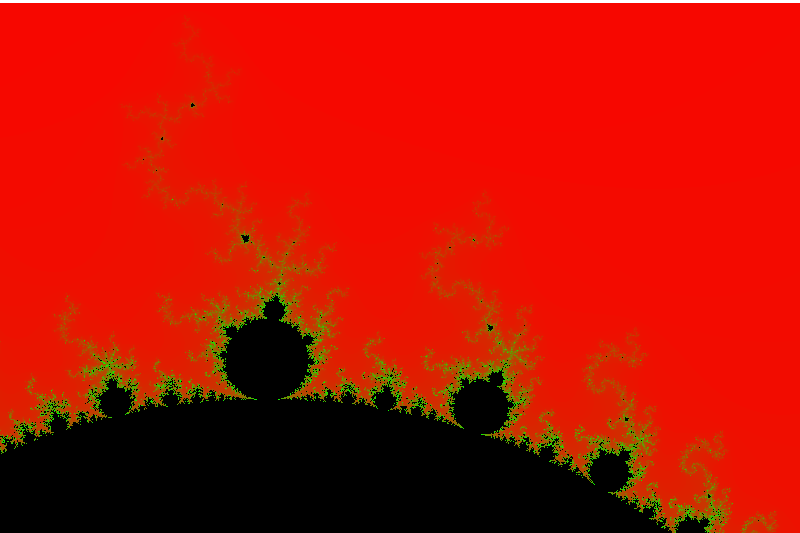
\includegraphics[scale=0.2]{mandelbrot.png} ~
    \begin{tabular}{|r|r|r|r|r|}
      \hline
      $N$  &t�ches & \ocaml{Cores} & \ocaml{Network} \\
      \hline\hline
      2       & 10 & 15.8       (1.86$\times$) &  20.3  (1.45$\times$)      \\
      & 30 & 15.7       (\emph{1.87}$\times$) &  18.7 (1.57$\times$)       \\
      & 100 & 16.1      (1.83$\times$) &  19.8   (1.48$\times$)    \\
      & 1000 & 19.6     (1.50$\times$) &  38.6    (0.76$\times$)  \\
      \hline
      4       & 10 & 9.50       (3.09$\times$)  &  14.4     (2.04$\times$)  \\
      & 30 & 8.26       (\emph{3.56}$\times$)  &  11.4  (2.58$\times$) \\
      & 100 & 8.37      (3.51$\times$)  &  11.4  (2.58$\times$) \\
      & 1000 & 10.6     (2.77$\times$)  &  20.5   (1.43$\times$) \\
      \hline
      8       & 10 & 9.40       (3.13$\times$)  &  12.6    (2.33$\times$)  \\
      & 30 & 4.24       (\emph{6.93}$\times$)  &   7.6  (3.87$\times$)    \\
      & 100 & 4.38      (6.71$\times$)  &   7.5    (3.92$\times$)  \\
      & 1000 & 6.86     (4.29$\times$)  &  11.3    (2.60$\times$)  \\
      \hline
    \end{tabular}
\end{frame}

\begin{frame}\frametitle{Case Study: Matrix Multiplication}
\end{frame}

\begin{frame}\frametitle{Conclusion}
  conclusion, future work, etc.
\end{frame}


\end{document}

%%% Local Variables: 
%%% mode: latex
%%% TeX-master: t
%%% End: 

